\documentclass{ximera}

\input{../preamble.tex}

\title{Multiplication with Integers}
\author{Vic Ferdinand, Betsy McNeal, Jenny Sheldon}

\begin{document}

\begin{abstract}
We look at multiplying integers.
\end{abstract}
\maketitle

\section{Activities for this section:}
\link[Our problems are multiplying]{https://ximera.osu.edu/m4t/elementaryActivities/SemesterOnePacket/elementaryActivities/Integers/OurProblemsAreMultiplying}


Now that we've conquered addition and subtraction, let's move on to multiplication.  The biggest difference between what we did with addition and subtraction and what we will do with multiplication is the units on each of the numbers. Remember that with addition and subtraction, all of the units are the same. But with multiplication, the units are different. For instance, compare and contrast the following examples.
\begin{center}
    $4$ (apples) + $9$ (apples) = $13$ (apples)
    
    $4$ (baskets of apples) $\times$ $9$ (apples per basket) = $36$ (apples)
\end{center}
We will need a different strategy for multiplication!

\section{Checks and Bills}

%As we have done previously, let's begin by looking at a multiplication problem with whole numbers, and then slowly introduce integers.  Remember to look back at our sections about multiplication in the text!
%
%\begin{question}
%Johnny has $9$ lunch bags, and each lunch bag has $2$ apples in it.  How many apples does Johnny have all together?
%
%\begin{prompt}
%As an expression involving the multiplication sign, Johnny has $\answer[given]{9 \times 2}$ apples.
%\end{prompt}
%\end{question}
%
%We can think of this problem as making $9$ copies of the $2$ apples per bag.  As a story about checks and bills, then, we could think of making $9$ copies of \$$2$.

We're jumping right in with an example using the repeated addition model of multiplication. In other words, when we write a story problem for $9 \times 2$, we are thinking about this as $9$ copies of the quantity $2$, or $2 + 2 + 2 + 2 + 2 + 2 + 2 + 2 + 2$.


\begin{example}
Let's write a checks and bills story problem for $9 \times 2$.  Johnny will still be our small business owner.  Starting with the second number, we know that these should be \wordChoice{\choice[correct]{checks} \choice{bills}}, each worth \$$2$, since the $2$ is positive.

We will use the first number to tell us whether Johnny is sending or receiving these checks. Since the $9$ is positive, we will say that that Johnny \wordChoice{\choice[correct]{receives} \choice{sends}} $9$ checks.


But what should be our question?  We could start by saying that Johnny's net worth is \$$0$, and ask what his net worth is now.  The natural answer to this question would be
\[
0 + (9\times 2) = 9 \times 2, 
\]
but that extra zero can feel a little bit confusing.

We might instead ask, ``How has Johnny's net worth changed?''  In this case, no matter 
what he had to start with, he now has $9 \times \$2$ {\em more} than he did previously.  Let's proceed with this second formulation, but cautiously.  We will need to make sure all of this still makes sense as we introduce negative numbers.

So, our story problem would be: Johnny receives $9$ checks each for $2$ dollars. How has his net worth changed? The answer would be that Johnny's net worth goes up by \$$18$, or the answer is $+18$ dollars.

\end{example}



Next, let's change the second number to be negative.
\begin{question}
Johnny receives $5$ bills, each for \$$10$.  After all bills are paid, how has Johnny's net worth changed?

\begin{prompt}
As an expression involving the multiplication sign, Johnny's net worth has changed by \$$\answer[given]{5}\times \answer[given]{-10}$.
\end{prompt}
\end{question}
Since Johnny is paying bills in this situation, it makes sense for his net worth to decrease, or for the change to be negative. Indeed, the change in his net worth is $-50$ dollars.

What if the number of groups is negative?  It may feel a little bit forced, but we will use the convention that a negative group means we are {\em sending} that many copies of our check or bill.  

\begin{example}
Johnny sends $3$ checks for \$$8$ each.  How has Johnny's net worth changed?

\begin{explanation}
Each of the checks is worth \$$8$, and there are $3$ of them.  This means that Johnny is sending out \$$\answer[given]{24}$.  In other words, his total net worth should be \$$\answer[given]{-24}$.  Since he is sending these, we have $-3$ groups, each with \$$8$ in them. In other words, this question can be solved by
\[
     \answer[given]{-3} \times \answer[given]{8}.
\]
\end{explanation}
\end{example}

%While beginning with a net worth of \$$0$ helps us to understand why negative groups might be represented by sending, this convention may still feel artificial.  Instead, we could ask the following.
%\begin{question}
%Johnny sends three checks, each for eight dollars.  How much has Johnny's net worth changed?
%
%\begin{prompt}
%Johnny's net worth has changed by \$$\answer[given]{(-3)} \times \answer[given]{8}$.
%\end{prompt}
%\end{question}
You might object that what we are doing here is actually calculating $3 \times 8$, and reasoning that the overall answer should be negative.  That's okay!  Remember that this concept is difficult, and we are doing the best we can to model difficult ideas.

\begin{question}
How would you write a checks and bills story to model $-22 \times -54$?
\begin{freeResponse}
We'd love to help with this in office hours if you aren't sure!
\end{freeResponse}
\end{question}

%Finally, let's look at what happens when we multiply two negatives together.
%\begin{question}
%Johnny sends $22$ bills, each for \$$54$.  After all bills are paid, how much has Johnny's net worth changed?
%
%\begin{prompt}
%Johnny's net worth has changed by \$$\answer[given]{(-22)} \times \answer[given]{(-54)}$.
%\end{prompt}
%\end{question}
%In terms of the situation with checks and bills, should this answer be positive or negative?  If Johnny is sending bills to other people, and then these other people pay their bills, this money comes back to Johnny.  So, his net worth overall should increase, meaning the change should be positive.  Notice that we didn't need to memorize any rules about negative numbers in order to come to this conclusion!
%


\section{Number Lines}

Next, let's use a number line to solve some multiplication problems with integers.  You can write 
a story problem to go along with each of these expressions for extra practice.

\begin{example}
Imagine using a number line like the one below to model the multiplication problem $5 \times (-3) $.
\begin{center}
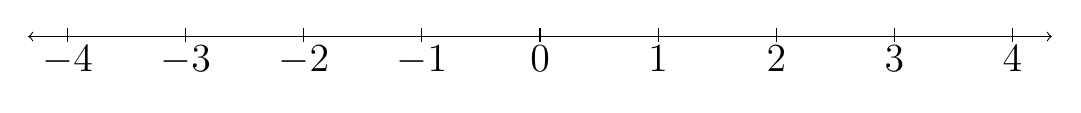
\begin{tikzpicture}[font=\Large]
\draw[<->] (-0.5,0) -- (12.5,0);
\foreach \x in {0,1.5, 3, 4.5, 6, 7.5, 9, 10.5,12}
\draw[shift={(\x,0)},color=black] (0pt,3pt) -- (0pt,-2pt);
\draw (0,0) node[below]{$-4$};
\draw (1.5,0) node[below]{$-3$};
\draw (3,0) node[below]{$-2$};
\draw (4.5,0) node[below]{$-1$};
\draw (6,0) node[below]{$0$};
\draw (7.5,0) node[below]{$1$};
\draw (9,0) node[below]{$2$};
\draw (10.5,0) node[below]{$3$};
\draw (12,0) node[below]{$4$};
\end{tikzpicture}  
\end{center}
We are still thinking about multiplication as repeated addition here: $5 \times -3$ should be five copies of $-3$.  As with our story problems, the question or starting point requires care.  Since we would like to investigate how our value changes after these jumps, it's natural to start on zero. If we think about $(-3) + (-3) + (-3) + (-3) + (-3)$, we 
are adding, so we will move \wordChoice{\choice[correct]{forward} \choice{backwards}}.  Now, the amount we are adding each time is $-3$, which is negative, so we will face  \wordChoice{\choice{right} \choice[correct]{left}}. Finally, we can think of the steps as our groups, meaning the amount we move with each step should be $\answer[given]{3}$ spaces. After taking $\answer[given]{5}$ such steps,  where on the number line are we now? 

\begin{prompt}
We are located at the tick labeled $\answer[given]{-15}$.
\end{prompt}
\end{example}

\begin{example}
Imagine using a number line like the one below to model the multiplication problem $(-8) \times (-7)$.
\begin{center}
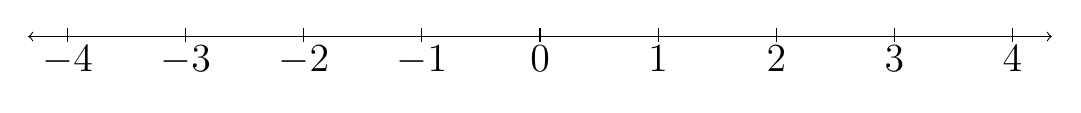
\begin{tikzpicture}[font=\Large]
\draw[<->] (-0.5,0) -- (12.5,0);
\foreach \x in {0,1.5, 3, 4.5, 6, 7.5, 9, 10.5,12}
\draw[shift={(\x,0)},color=black] (0pt,3pt) -- (0pt,-2pt);
\draw (0,0) node[below]{$-4$};
\draw (1.5,0) node[below]{$-3$};
\draw (3,0) node[below]{$-2$};
\draw (4.5,0) node[below]{$-1$};
\draw (6,0) node[below]{$0$};
\draw (7.5,0) node[below]{$1$};
\draw (9,0) node[below]{$2$};
\draw (10.5,0) node[below]{$3$};
\draw (12,0) node[below]{$4$};
\end{tikzpicture}  
\end{center}
We begin by standing on the number line at the tick marked with $\answer[given]{0}$.  Since our groups are negative, we can think of this as subtracting our copies of $-7$, so we will move 
\wordChoice{\choice{forward} \choice[correct]{backward}}, and take $\answer[given]{8}$ total steps.  We will face \wordChoice{\choice{right} 
\choice[correct]{left}}, because $-7$ is negative, and each step will move  $\answer[given]{7}$ spaces.  Where on the number line are we now? 

\begin{prompt}
We are located at the tick labeled $\answer[given]{56}$.
\end{prompt}
\end{example}

Notice again that if we multiply two negative numbers, we face backwards while moving backwards, for a net result of moving in the positive direction along the number line.  %Try this out with some friends if you are skeptical.

We encourage you to try out using red and black chips to model some multiplication problems, and to investigate using patterns as we did with addition and subtraction. However, since our in-class work will focus mostly on addition and subtraction, we'd like to end this section with a few comments about division.



%\section{Patterns}
%
%Finally, we investigate subtraction of negative numbers via patterns.
%\begin{example}
%Consider the sequence of addition problems.
%\begin{align*}
%5 \times 4 &= \answer[given]{20} \\
%5 \times 3 &= \answer[given]{15} \\
%5 \times 2 &= \answer[given]{10} \\
%5 \times 1 &= \answer[given]{5} \\
%5 \times 0 &= \answer[given]{0}
%\end{align*}
%As we move down the chart, moving one row down results in the final answer decreasing by 
%$\answer[given]{5}$.  So, if the pattern continues to hold, we expect the answer to 
%$5 \times (-1)$ to be $\answer[given]{-5}$, since it is five less than $0$.
%\end{example}
%If we are convinced by this pattern that a positive number times a negative number should be negative, we can use the commutative property to convince ourselves that a negative number times a positive number should also be negative.  Then, we can use our patterns again to convince ourselves that a negative number times a negative number should be positive.
%\begin{example}
%Consider the sequence of addition problems.
%\begin{align*}
%-5 \times 4 &= \answer[given]{-20} \\
%-5 \times 3 &= \answer[given]{-15} \\
%-5 \times 2 &= \answer[given]{-10} \\
%-5 \times 1 &= \answer[given]{-5} \\
%-5 \times 0 &= \answer[given]{0}
%\end{align*}
%As we move down the chart, moving one row down results in the final answer increasing by 
%$\answer[given]{5}$.  So, if the pattern continues to hold, we expect the answer to 
%$-5 \times (-1)$ to be $\answer[given]{5}$, since it is five more than $0$.
%\end{example}
%
%\subsection{Extra Examples}
%Since multiplication with negatives is a complicated topic, here are two extra ways to think about this concept.  First, we will talk about algebra, and second we will use a more advanced physical model.
%
%We mentioned very briefly when talking about patterns that the properties of addition and subtraction can help us to understand multiplication with negative numbers.  
%
%\begin{example}
%We can model multiplication problems like $2 \times (-17)$ without much trouble.  In fact, most of our trouble came from attempting to understand what negative groups should mean.  If we instead wanted to consider $(-17) \times 2$, we might quickly realize that the commutative property of multiplication gives us 
%\[
%(-17) \times 2 = \answer[given]{2} \times \answer[given]{-17}, 
%\]
%which we could model with a story, a number line, or chips.  Notice, however, that we're making use of the idea that a positive number multiplied by a negative number gives us a negative answer overall -- and this fact requires justification some other way!
%\end{example}
%
%Earlier in this section, our justification for why a positive number multiplied by a negative number is a negative number came mostly from describing the multiplication in a way we could understand or represent with a physical situation.  Even number lines could be thought of as a physical situation, since we can use our bodies to move along the lines.  Patterns are the beginning of looking at this concept algebraically, and let's now do some more advanced algebra.
%
%We know that if we have a negative number, like $-17$, we can write this as $(-1) \times 17$.  Algebraically, why should this be true?  We want our negative numbers to represent the opposite of our positive numbers.  If Sue has $-17$ dollars, she needs to obtain $17$ more dollars to make it back to zero.  If Sam is standing on the tick labeled $-17$, he needs to move $17$ spaces to the right to get back to zero.  In other words, $-17$ should satisfy the equation 
%\[17 + (-17) = 0.\]
%
%What about $(-1) \times 17$?
%\begin{example}
%Let's look at $(-1) \times 17$ to see if this is really equal to $-17$.  If so, when we add $17$ to $(-1) \times 17$, we should get back to $0$.
%\[
%(-1) \times 17 + 17 = ?
%\]
%First, we see that there is a $17$ in each of these terms, so let's factor it out.
%\[
%\answer[given]{17} \left ( \answer[given]{-1} + \answer[given]{1} \right ) = ?
%\]
%Inside the parenthesis, we should now know what to do.
%\[
%\answer[given]{17} \left ( \answer[given]{0} \right ) = \answer[given]{0}
%\]
%\end{example}
%
%This may seem a little silly, but understanding and developing good rules for using negative numbers with algebra was a concern of many mathematicians before negative numbers were fully accepted.  
%
%There is actually one extra fact we have used in the previous argument that you may have noticed.  To really be sure that $(-1) \times 17 = -17$, we should really be sure that the only number we can add to $17$ to get zero is $-17$.  Proving this fact is possible, but we won't look at that proof in this course.  
%
%Now that we know that we can write a negative number as $-1$ multiplied by the positive version of that number, we can use more of our properties.
%
%\begin{example}
%Use the associative property of multiplication and the fact that $-17 = (-1) \times 17$ to make sense of $(-17) \times 2$.
%\begin{explanation}
%\[
%(-17) \times 2 = \left ( (-1) \times \answer[given]{17} \right ) \times 2 = (-1) \times \left ( \answer[given]{17} \times \answer[given]{2} \right )
%\]
%We have plenty of practice computing $17 \times 2$, and this algebra shows us why $(-17) \times 2$ is the negative of $17 \times 2$.
%\end{explanation}
%%This technique gets a little less useful, however, with things like $(-2) \times (-17)$.
%%\begin{align*}
%%    (-2) \times (-17) &= (-1)\left( \answer[given]{2} \right ) \times (-1) \times \left ( \answer[given]{17}\right ) \\
%%    & = (-1) \times \left ( \answer[given]{2} \times \left ( (-1) \answer[given]{17} \right ) \right ) \\
%%    & = (-1) \times \left ( \left (\answer[given]{2} \times  (-1) \right ) \times \answer[given]{17} \right ) \\
%%    & = (-1) \times \left ( \left ((-1) \times \answer[given]{2} \right ) \times \answer[given]{17} \right ) \\
%%    & = (-1) \times \left ( (-1) \times \left (\answer[given]{2} \times \answer[given]{17} \right ) \right ) \\
%%    &= \left ((-1) \times (-1) \right ) \times \left ( \answer[given]{2} \times \answer[given]{17} \right )
%%\end{align*}
%%Again, as long as we understand what to do with $(-1)(-1)$, we have plenty of practice computing $2 \times 17$.
%\end{example}
%
%Let's now move to a different kind of model for multiplication.
%
%\begin{example}
%You might recall the equation
%\[
%\text{Distance} = \text{Time} \times \text{Rate}.
%\]
%Let's say that zero is our position at noon, and we have been traveling east on an east-west highway at a steady rate of $50$ miles per hour.  Where were we at $9$am?
%
%Notice that $9$am was three hours ago, and so this question is equivalent to asking for the solution to $(-3) \times 50$.  Knowing that the answer is $\answer[given]{-150}$, we should interpret this result to say that at $9$am, we were $\answer[given]{150}$ miles \wordChoice{\choice{east} \choice[correct]{west}} of where we were at noon.
%\end{example}
%

\section{Division}

Remember that we defined division as the inverse of multiplication, so we will use what we know about multiplication to think about division. We have used our models to explain why the following rules make sense.
\begin{itemize}
	\item Multiplying two positive numbers gives a positive result.
	\item Multiplying one positive and one negative number gives a negative result.
	\item Multiplying two negative numbers gives a positive result.
\end{itemize}  
Let's use this to think about a division problem.

\begin{example}
What is $24 \div (-6)$?

We can think of $24 \div (-6)$ as a multiplication problem by using
\[
(-6) \times ? = 24
\]
or
\[
? \times (-6) = 24.
\]
While which problem we choose matters in our stories, the \wordChoice{\choice{associative} \choice[correct]{commutative} \choice{distributive}} property of multiplication gives us the same answer in either case.  We also know from our work with multiplication that the sign of the answer must be \wordChoice{\choice{positive} \choice[correct]{negative}}.  Since $24 \div 6 = \answer[given]{4}$, we now know that $24 \div (-6)$ should equal $\answer[given]{-4}$.

If we wanted to write a story problem using checks and bills for $(-6) \times ? = 24$, we could do the following. Johnny sent $6$ identical items in the mail, and his net worth changed by \$$24$. What was the value of each item that was sent?

Notice that the answer to this question is that Johnny must have sent bills (so his net worth would go up from sending something), and these bills must have been for \$$4$ each, so that the total change is \$$24$.



\end{example}



As we have stated throughout, this is a complicated concept.  You may need to work through the examples several times, as well as ask questions, before understanding completely.  Don't worry, though -- many of history's most notable mathematicians shared these struggles!



\end{document}

